\documentclass[11pt]{article}
\usepackage{geometry}
\geometry{a4paper, margin=0.75in}
\usepackage{enumitem}
\usepackage{hyperref}
\usepackage[dvipsnames]{xcolor}

\usepackage{epigraph}

\usepackage{multicol}
\usepackage{tikz}
\usepackage{pgfplots}
\pgfplotsset{compat=1.18}

\begin{document}

% 背景浮水印层 - 简化版本,更容易显示
\begin{tikzpicture}[remember picture, overlay]
    % 定义颜色
    \definecolor{watermarkblue}{RGB}{0, 122, 255}
    \definecolor{watermarkgray}{RGB}{142, 142, 147}
    \definecolor{watermarklight}{RGB}{200, 200, 220}
    
    % 设置透明度 - 更明显的透明度
    \tikzset{watermark/.style={opacity=0.15, thin}}
    
    % 简单的电路图案 - 左上角
    \begin{scope}[watermark, color=watermarkblue]
        \draw (0.5, 9.5) rectangle (2.5, 10.5);
        \draw (0.5, 9.5) -- (2.5, 9.5);
        \draw (0.5, 10) -- (2.5, 10);
        \draw (0.5, 10.5) -- (2.5, 10.5);
        \draw (1, 9.5) -- (1, 10.5);
        \draw (1.5, 9.5) -- (1.5, 10.5);
        \draw (2, 9.5) -- (2, 10.5);
        \fill (0.5, 9.5) circle (0.05);
        \fill (2.5, 9.5) circle (0.05);
        \fill (0.5, 10.5) circle (0.05);
        \fill (2.5, 10.5) circle (0.05);
    \end{scope}
    
    % 简单的大脑图案 - 右上角
    \begin{scope}[watermark, color=watermarkgray]
        \draw (6.5, 9.5) .. controls (7, 10) and (7.5, 10) .. (8, 9.5)
              .. controls (8.5, 9) and (8.5, 8.5) .. (8, 8)
              .. controls (7.5, 7.5) and (7, 7.5) .. (6.5, 8)
              .. controls (6, 8.5) and (6, 9) .. (6.5, 9.5);
        \draw (6.7, 9.3) -- (7.3, 9.1);
        \draw (6.8, 8.8) -- (7.2, 8.6);
        \draw (6.9, 8.3) -- (7.1, 8.1);
    \end{scope}
    
    % 简单的原子图案 - 左下角
    \begin{scope}[watermark, color=watermarklight]
        \fill (0.5, 1.5) circle (0.2);
        \draw[dashed] (0.5, 1.5) circle (0.8);
        \draw[dashed] (0.5, 1.5) circle (1.2);
        \fill (0.5, 2.3) circle (0.08);
        \fill (1.3, 1.5) circle (0.08);
        \fill (0.5, 0.7) circle (0.08);
        \fill (1.7, 1.5) circle (0.08);
    \end{scope}
    
    % 简单的芯片图案 - 右下角
    \begin{scope}[watermark, color=watermarkblue]
        \draw (6.5, 1.5) rectangle (8.5, 3.5);
        \draw (6.7, 1.7) rectangle (8.3, 3.3);
        \draw (6.5, 2) -- (6.3, 2);
        \draw (6.5, 2.5) -- (6.3, 2.5);
        \draw (6.5, 3) -- (6.3, 3);
        \draw (8.5, 2) -- (8.7, 2);
        \draw (8.5, 2.5) -- (8.7, 2.5);
        \draw (8.5, 3) -- (8.7, 3);
    \end{scope}
    
    % 简单的神经网络 - 中央
    \begin{scope}[watermark, color=watermarkblue]
        \fill (4, 6) circle (0.1);
        \fill (4, 5.5) circle (0.1);
        \fill (4, 5) circle (0.1);
        \fill (5, 6) circle (0.1);
        \fill (5, 5.5) circle (0.1);
        \fill (5, 5) circle (0.1);
        \fill (6, 5.5) circle (0.1);
        \draw (4, 6) -- (5, 6);
        \draw (4, 6) -- (5, 5.5);
        \draw (4, 6) -- (5, 5);
        \draw (4, 5.5) -- (5, 6);
        \draw (4, 5.5) -- (5, 5.5);
        \draw (4, 5.5) -- (5, 5);
        \draw (4, 5) -- (5, 6);
        \draw (4, 5) -- (5, 5.5);
        \draw (4, 5) -- (5, 5);
        \draw (5, 6) -- (6, 5.5);
        \draw (5, 5.5) -- (6, 5.5);
        \draw (5, 5) -- (6, 5.5);
    \end{scope}
    
    % 简单的数学符号 - 分散分布
    \begin{scope}[watermark, color=watermarkgray]
        % 积分符号
        \draw (2, 7) -- (2, 8);
        \draw (1.8, 7) -- (2.2, 7);
        \draw (1.8, 8) -- (2.2, 8);
        
        % 求和符号
        \draw (7, 7) circle (0.2);
        \draw (6.8, 7) -- (7.2, 7);
        \draw (7, 6.8) -- (7, 7.2);
        
        % 矩阵
        \draw (3, 2.5) rectangle (4, 3.5);
        \draw (3.2, 2.5) -- (3.2, 3.5);
        \draw (3.4, 2.5) -- (3.4, 3.5);
        \draw (3.6, 2.5) -- (3.6, 3.5);
        \draw (3.8, 2.5) -- (3.8, 3.5);
        \draw (3, 2.7) -- (4, 2.7);
        \draw (3, 2.9) -- (4, 2.9);
        \draw (3, 3.1) -- (4, 3.1);
        \draw (3, 3.3) -- (4, 3.3);
    \end{scope}
    
    % 量子比特 - 中上方
    \begin{scope}[watermark, color=watermarklight]
        \draw (4, 8.5) circle (0.15);
        \draw (4.5, 8.5) circle (0.15);
        \draw (5, 8.5) circle (0.15);
        \draw[dashed] (4, 8.5) -- (4.5, 8.5);
        \draw[dashed] (4.5, 8.5) -- (5, 8.5);
    \end{scope}
\end{tikzpicture}

\begin{center}
    \LARGE \textbf{Kevin Ting-Kai Kuo}
\end{center}

\vspace{1em}

% \section*{Contact Information}
\begin{multicols*}{2}
    


% \columnbreak
% % \section*{Motto}
% \epigraph{Think different, connect the dots.}{\textit{Steve Jobs}}

% {\footnotesize I am familiar with solving\textbf{ classical and quantum optical models}, numerically/symbolically, for instance (but not limited to):
%     • Jaynes-Cumming model for two-photon strongly-correlated system. • Bosonic sampling approach to implement optical quantum computation • Using \textbf{FDTD} to simulate optical metamaterial camera lens in Tyrafos technology.\\}

% \hrule

\section*{Contact}
{\footnotesize
\begin{itemize}[noitemsep]
    \item \href{https://github.com/Kuo-TingKai}{\textbf{\textcolor{blue}{Github}}}
    \item \textbf{Phone:} +886-922-082-811
    \item \textbf{Email:} KaiCoCat@proton.me
    \item \href{https://medium.com/@nehsm30126}{\textbf{\textcolor{blue}{Medium}}} 
    \item \href{https://www.overleaf.com/read/xzdtxtgxtnby#49163b}{\textbf{\textcolor{blue}{Article List}}}
    \item \href{https://github.com/Kuo-TingKai/theorem-dream}{\textbf{\textcolor{blue}{The interactive website of my micro-novel}}}
\end{itemize}
}

\section*{Fast Navigation}
You can jump to \href{#software-dev}{\textbf{\textcolor{blue}{Software Development}}} and \href{#experience}{\textbf{\textcolor{blue}{Experience}}} section\\

\hrule

\section*{Technology Stack Dashboard}
\begin{center}
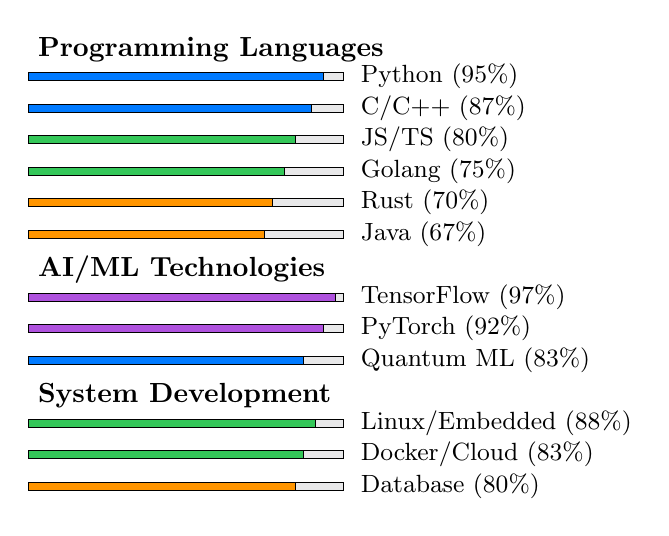
\begin{tikzpicture}[scale=0.5]
    % 定义颜色
    \definecolor{techblue}{RGB}{0, 122, 255}
    \definecolor{techgreen}{RGB}{52, 199, 89}
    \definecolor{techorange}{RGB}{255, 149, 0}
    \definecolor{techred}{RGB}{255, 59, 48}
    \definecolor{techpurple}{RGB}{175, 82, 222}
    \definecolor{techgray}{RGB}{142, 142, 147}
    
    % 编程语言技能条
    \node[anchor=west] at (-2, 4.0) {\textbf{Programming Languages}};
    
    \draw[fill=techgray!20] (-2, 3.2) rectangle (6, 3.4);
    \draw[fill=techblue] (-2, 3.2) rectangle (5.5, 3.4);
    \node[anchor=west] at (6.2, 3.3) {\small Python (95\%)};
    
    \draw[fill=techgray!20] (-2, 2.4) rectangle (6, 2.6);
    \draw[fill=techblue] (-2, 2.4) rectangle (5.2, 2.6);
    \node[anchor=west] at (6.2, 2.5) {\small C/C++ (87\%)};
    
    \draw[fill=techgray!20] (-2, 1.6) rectangle (6, 1.8);
    \draw[fill=techgreen] (-2, 1.6) rectangle (4.8, 1.8);
    \node[anchor=west] at (6.2, 1.7) {\small JS/TS (80\%)};
    
    \draw[fill=techgray!20] (-2, 0.8) rectangle (6, 1.0);
    \draw[fill=techgreen] (-2, 0.8) rectangle (4.5, 1.0);
    \node[anchor=west] at (6.2, 0.9) {\small Golang (75\%)};
    
    \draw[fill=techgray!20] (-2, 0.0) rectangle (6, 0.2);
    \draw[fill=techorange] (-2, 0.0) rectangle (4.2, 0.2);
    \node[anchor=west] at (6.2, 0.1) {\small Rust (70\%)};
    
    \draw[fill=techgray!20] (-2, -0.8) rectangle (6, -0.6);
    \draw[fill=techorange] (-2, -0.8) rectangle (4.0, -0.6);
    \node[anchor=west] at (6.2, -0.7) {\small Java (67\%)};
    
    % AI/ML 技能条
    \node[anchor=west] at (-2, -1.6) {\textbf{AI/ML Technologies}};
    
    \draw[fill=techgray!20] (-2, -2.4) rectangle (6, -2.2);
    \draw[fill=techpurple] (-2, -2.4) rectangle (5.8, -2.2);
    \node[anchor=west] at (6.2, -2.3) {\small TensorFlow (97\%)};
    
    \draw[fill=techgray!20] (-2, -3.2) rectangle (6, -3.0);
    \draw[fill=techpurple] (-2, -3.2) rectangle (5.5, -3.0);
    \node[anchor=west] at (6.2, -3.1) {\small PyTorch (92\%)};
    
    \draw[fill=techgray!20] (-2, -4.0) rectangle (6, -3.8);
    \draw[fill=techblue] (-2, -4.0) rectangle (5.0, -3.8);
    \node[anchor=west] at (6.2, -3.9) {\small Quantum ML (83\%)};
    
    % 系统开发技能条
    \node[anchor=west] at (-2, -4.8) {\textbf{System Development}};
    
    \draw[fill=techgray!20] (-2, -5.6) rectangle (6, -5.4);
    \draw[fill=techgreen] (-2, -5.6) rectangle (5.3, -5.4);
    \node[anchor=west] at (6.2, -5.5) {\small Linux/Embedded (88\%)};
    
    \draw[fill=techgray!20] (-2, -6.4) rectangle (6, -6.2);
    \draw[fill=techgreen] (-2, -6.4) rectangle (5.0, -6.2);
    \node[anchor=west] at (6.2, -6.3) {\small Docker/Cloud (83\%)};
    
    \draw[fill=techgray!20] (-2, -7.2) rectangle (6, -7.0);
    \draw[fill=techorange] (-2, -7.2) rectangle (4.8, -7.0);
    \node[anchor=west] at (6.2, -7.1) {\small Database (80\%)};
    

    

\end{tikzpicture}
\end{center}

\section*{Experience}\label{experience}

% 时间轴样式
\begin{tikzpicture}[remember picture, overlay]
    % 定义颜色
    \definecolor{timelineblue}{RGB}{0, 122, 255}
    \definecolor{timelinegray}{RGB}{142, 142, 147}
    
    % 主时间轴线 - 调整位置和长度
    \draw[timelineblue, thick] (-0.8, 0.5) -- (-0.8, -18);
    
    % 时间节点和连接线 - 重新调整位置
    % 2024 Sep - now
    \fill[timelineblue] (-0.8, 0.5) circle (3pt);
    \draw[timelineblue, thick] (-0.8, 0.5) -- (-0.6, 0.5);
    
    % 2023 Dec - 2024 July
    \fill[timelineblue] (-0.8, -3.5) circle (3pt);
    \draw[timelineblue, thick] (-0.8, -3.5) -- (-0.6, -3.5);
    
    % 2023 Jan - Dec
    \fill[timelineblue] (-0.8, -7.5) circle (3pt);
    \draw[timelineblue, thick] (-0.8, -7.5) -- (-0.6, -7.5);
    
    % 2022 Sep - Dec
    \fill[timelineblue] (-0.8, -11.5) circle (3pt);
    \draw[timelineblue, thick] (-0.8, -11.5) -- (-0.6, -11.5);
    
    % 2022 Mar - Jul
    \fill[timelineblue] (-0.8, -14.5) circle (3pt);
    \draw[timelineblue, thick] (-0.8, -14.5) -- (-0.6, -14.5);
    
    % 2020 Jul - 2022 Jan
    \fill[timelineblue] (-0.8, -17.5) circle (3pt);
    \draw[timelineblue, thick] (-0.8, -17.5) -- (-0.6, -17.5);
    
    % 时间标签 - 重新调整位置
    \node[anchor=east, font=\tiny, color=timelinegray] at (-1.0, 0.5) {2024};
    \node[anchor=east, font=\tiny, color=timelinegray] at (-1.0, -3.5) {2023-24};
    \node[anchor=east, font=\tiny, color=timelinegray] at (-1.0, -7.5) {2023};
    \node[anchor=east, font=\tiny, color=timelinegray] at (-1.0, -11.5) {2022};
    \node[anchor=east, font=\tiny, color=timelinegray] at (-1.0, -14.5) {2022};
    \node[anchor=east, font=\tiny, color=timelinegray] at (-1.0, -17.5) {2020-22};
\end{tikzpicture}

\vspace{0.5em}

\subsection*{Senior engineer, IKG Team, 2024 Sep. - now}
\begin{itemize}[noitemsep]
    \item Develope browser-end multimedia player for video streams using FFmpeg, WebGPU,WebAssembly, accelerating streams with \textbf{NVIDIA encoder} and customizing\textbf{ AI-masking frames} from SRS\textbf{ mediaserver} 
    \item Authentication for stream requests
    \item Serial port communication (USB, RS232) for game machine \textbf{micro-controller(MCU)}
    \item Object storages for VODs with Tencent/BytePlus cloud services
    \item Websockets/MQTT for game state machine message passing to Database (\textbf{PostgreSQL, MongoDB})
    \item \textbf{Monitoring/Logging/Telemetry} for network TTFF/latency with Prometheus, google analytics, Sentry \textbf{on cloud server}
    \item Monte Carlo for event simulations.
    \item Technology stacks: Python/C++/\\Typescript/JavaScript/Go 
    \item Documenting with \textbf{Confluence}
    \item \textbf{Co-working with Europe team} for game projects
\end{itemize}

\vspace{0.8em}

\subsection*{Senior engineer, Arcadyan Technology Co. Ltd., 2023 Dec.- 2024 July }
\begin{itemize}[noitemsep]
    \item Google xTS test suite for Android TV development, deployed and ran on Ubuntu Linux server
    \item Test automation cluster build-up (24-48 physical devices) for passing over 1-million test cases nightly by \textbf{sharding}.
    \item \textbf{Leadership:} Dispatch/Schedule remote contractors to complete a xTS test suite cycle per week
    \item \textbf{OTA/eMMC firmware update}
\end{itemize}

\vspace{0.8em}

\subsection*{Senior engineer, Marvell Technology Co. Ltd., 2023 Jan.-Dec.}
\begin{itemize}[noitemsep]
    \item SSD NVMe protocol front-end test/simulation tool development/test for \textbf{SSD controller firmware}, including device enumeration,function level hot reset features\textbf{ for cloud server storage}
    \item Test tool GUI development with PySide2
    \item Used qTest for regression test documenting, Jfrog for constructing CI upstream and software release. CI/CD and release.Wrote Java/Groovy/Shell scripts for CI/CD code on Jenkins.
    \item Docker/Manylinux to make software release more portable
    \item Slack/Jira for agile development
\end{itemize}

\vspace{0.8em}

\subsection*{Software Freelancer, 2022 Sep.-Dec.}
\begin{itemize}[noitemsep]
    \item AI pose detection for body training posing correction with PoseNet.
\end{itemize}

\vspace{0.8em}

\subsection*{\textbf{Algorithm engineer}, Tyrafos Technology, 2022 Mar.-Jul.}
\begin{itemize}[noitemsep]
    \item Real-time face recognition/fingerprint verification on embedded devices using neural network quantization in TF-lite
    \item Real-time Image signal processing (ISP) such like HDR, 3A on mobile camera in OpenCV
    \item Optical TRNG encryption module on mobile phones obeying NIST entropy extraction test suite
\end{itemize}

\vspace{0.8em}

\subsection*{Full-stack engineer and Co-founder, Eunomia (a legal-tech startup), 2020 Jul.- 2022 Jan.}
\begin{itemize}[noitemsep]
    \item Build-up the GUI of a document editor with Sequence-to-Sequence model with PyTorch for NLP core, for the purpose of collaboration with lawyers and other workers in legal industry. Our WebUI was implemented with Vue.js/Quill.js, deployed on GCP/Firebase.
    \item Obtained the 2nd place in the 1st Lawsnote Legaltech Hackathon, 2020, Taiwan.
    \item Assisted by NCCU innovation center start-up incubator.
\end{itemize}

\hrule

\section*{Skills}
% A brief summary of your skills, exper, ience, and career goals.
\subsection*{Programming Languages}
% Todo 替以下Rust加上此超連結 https://github.com/xiph/rav1e/compare/master...Kuo-TingKai:rav1e:master
\begin{itemize}[noitemsep]
    \item \href{https://github.com/Kuo-TingKai/submarine-cable-monitor}{\textbf{\textcolor{blue}{Python}}}, 
    \href{https://github.com/Kuo-TingKai/cpp_linux_chat}{\textbf{\textcolor{blue}{C/C++}}}, 
    \href{https://github.com/Kuo-TingKai/three-3d-game}{\textbf{\textcolor{blue}{Javascript/Typescript}}}, 
    \href{https://github.com/Kuo-TingKai/golang-web3-app}{\textbf{\textcolor{blue}{Golang}}},
    \href{https://github.com/xiph/rav1e/compare/master...Kuo-TingKai:rav1e:master}{\textbf{\textcolor{blue}{Rust}}},
    \href{https://github.com/Kuo-TingKai/java-backend-cloud-maven-app}{\textbf{\textcolor{blue}{Java}}}, 
    \href{https://github.com/Kuo-TingKai/lean4-basic-ag}{\textbf{\textcolor{blue}{Lean}}}, PHP, 
    \href{https://github.com/Kuo-TingKai/RoR-app}{\textbf{\textcolor{blue}{Ruby on Rails}}}, 
    Julia, Shell scripts, Mathematica, R
\end{itemize}

\subsection*{Working OS Platforms}
\begin{itemize}[noitemsep]
    \item Ubuntu Linux, CentOS Linux, Android Linux, RaspberryPi OS, Windows
\end{itemize}

\subsection*{DL/ML/HPC/Statatistics}

\subsubsection*{DL Frameworks/AI compiler}
\begin{itemize}[noitemsep]
    \item Tensorflow:\href{https://github.com/Kuo-TingKai/TNNN}{\textbf{\textcolor{blue}{TF}}}/TF-lite/\\Tensornetwork/Tensorboard/\\Tensorflow C++ API\\
    Jax
    \item Pytorch: torch/torch\_geometric
    \item ONNX, MLIR
    \item HPC tools: Pybind11/BLAS/OpenMP 
\end{itemize}
\subsubsection*{Algorithms}
\begin{itemize}[noitemsep]
    \item ML/DL theory\\ Especially, I am sophisticated at a family of \textbf{physics-inspired} algorithms called tensor network (also called tensor-train decomposition,TT, or higher order singular value decomposition, HOSVD), which are used in \textbf{LoRA in the LLM} field. 
    \item Image signal processing (ISP) \\
    Edge CV using pre-trained NN models then fine-tuned/migrate learning to in-firm data,\textbf{ quantized to FP int8 }and deployed on RK3399 SoC equipped with camera lens collaboratively RD with FocalTech, for the face verification system.\\
    HDR tonemapping, color space conversion for CIS camera lens ISP pipeline (with OpenCV). Spherical aberration calibration for the robotic vacuum. \\
    Circle/edge detection for the eye-moving instrument.  
    \item \textbf{Quantum Machine Learning}\\ quantum-classical\textbf{ hybrid CNN architecture} implemented with Google Qiskit/Tensorflow/Pannylane/Strawberryfield running on IBMQ quantum server for solving the ground state energy of the molecule in the IBMQ Quantum Computing Hackathon.\\
    \item \textbf{Statistics}\\ multivariate time series such like ARIMA model, VAR, GARCH etc, with ARIMA(R) and Statsmodel(Python). Currently I am interested in the generalized version of AIC/BIC call WAIC/WBIC using algebraic statistics (algebraic geometry + statistics) invented by Watanabe, Riken.
    \item Numerical methods\\tensorization/Monte Carlo/Quantum Monte Carlo/Markov Chain Monte Carlo/Simulated annealing for solving combinatorical problem, e.g. the variant of travelling saleman problem (TSP) called QAOA, and physics problem ( phase transition classification and ground state solution).
    \item Cryptography: randomness(entropy) extraction, optical-based TRNG implemented by LED packaged on circuit for the electric network data transfer, which was inspired by Samsung mobile phone hardware encryption module.
\end{itemize}

\section*{Software Development}\label{software-dev}
\begin{itemize}[noitemsep]
    \item Profiler: perfetto/logcat/protobuf on Android Linux platform.
    \item \textbf{Real time, Low latency System design on Linux}: NVMe SSD controller tool development and test for several Linux distributions (Ubuntu/CentOS/RPI) using Pybind11 for binding top python API to C++ core library to call the NVMe/PCIe syscalls to the Linux kernel. Besides, we replaced the original ring buffer backend of  NVMe devices with IOUring/Liburing for better I/O performance.
    \item Web: Vue/Node/Django/GCP/Firebase
    \item Emulator/Simulator:Qemu(open-source)/\\AVD(Android)/Simics(Windriver) for SSD device development and test.
    \item GUI: PyQt5, PySide2
    \item \textbf{Cloud Container virtualization:Docker and Docker-compose}, LXC(Linux generic container technology), Proxmox
    \item OpenTelemetry for monitoring/logging/telemetry:\\ Prometheus/Grafana/Datadog/Sentry
    \item \textbf{Database: PostgreSQL, MongoDB}
    \item Agile: Scrum, Jira
\end{itemize}

\section*{Test}
\begin{itemize}[noitemsep]
    \item CI/CD: Jenkins/Groovy/Git action
    \item Test automation framework: Pytest/Postman/\\Selemium
\end{itemize}

\hrule

\section*{Education}

\subsection*{BA, Economics, National Chengchi University, 2016-2018}

    \begin{itemize}[noitemsep]
        \item RA (Ministry of Science and Technology), Taiwan Policy Center, 2017-2018
        \item Graduate/undergraduate maths courses: advanced calculus, stochastic process, advanced probability, stochastic PDE (2016 summer school, NTU), differential geometry
        \item Graduate/undergraduate econ courses: Financial time series, Econometrics, Game theory, Macroeconomics, Microeconomics
        \item TWSIAM conference 2018, poster paper, forecasting for win rate of NBA teams using HMM model with Dirichlet prior implemented by R
    \end{itemize}


\subsection*{MA, Economics, National Chengchi University, 2018-2019 (incomplete)}

    \begin{itemize}[noitemsep]
        \item ICAPE 2020 Conference (San Diego), oral presentation: \textit{Shinn-Shyr Wang, Ting-Kai Kuo and Wen-Chieh Lee, National Chengchi University: Combating thick polar networks: is there any effective way other than the strategic network formation?} Contribution: theoretical proof/numerical simulation for studying opinion convergence speed of manipulated social networks with echo-chamber effect implemented by Networkx and Numpy. I also set-up a manipulated chatroom with Node.js and Firebase providing for experimenters to use and monitored the opinion dynamics from the back-end.
        \item TA, principle of economics, 2018 autumn
    
        \item \textbf{RA, Music and Culture Technology Lab, Institute of Information Science, Academia Sinica, 2019}: Music score learning using graph neural network and topological data analysis with Tensorflow, Scikit-learn, Librosa.
        
    \end{itemize}

\subsection*{MA, Applied Physics, National Chengchi University, 2019-2020 (incomplete, master thesis defense passed)}

    \begin{itemize}[noitemsep]
        \item RA, Condensed Matter Center, NTU/ Institute of Applied Physics, NCCU
        \item TA, computational physics, 2019 spring, teaching quantum Monte Carlo
        \item Research: tensorize neural networks on condensed matter physics and conventional supervised learning task (image recognition) implemented by Tensorflow/Keras/Tensornetwork
        \item Courses: quantum computing, quantum mechanics, statistical mechanics, computational physics
        \item Seminar project: implemented quantum exponential adder with qiskit in quantum computing course 
    \end{itemize}

\hrule

\section*{Math/Physics/TCS Research Interest}
\begin{itemize}[noitemsep]
    \item Mathematica/Sagemath(Python) for symbolic/numerical computation for the Mathematical Physics.
    \item Computer Automatic Proof in Lean4/Coq/\\Isabelle language.  
    \item \textbf{ Currently, I am working with Dr. \href{https://www.bing.com/search?q=en-jui+kuo&gs_lcrp=EgZjaHJvbWUqBggBEEUYOzIGCAAQRRg5MgYIARBFGDsyBggCEEUYOzIGCAMQRRg7MgYIBBAAGEAyBggFEAAYQDIGCAYQRRg9MgYIBxBFGDwyBggIEEUYPNIBCDE2NjVqMGoxqAIAsAIA&FORM=ANAB01&PC=HCTS}{Kuo, En-Jui (UMD)} and Dr. \href{https://scholar.google.com.hk/citations?user=38TPAxMAAAAJ&hl=en}{Kam, Chon-Fai (SUNY Buffalo)} with: (1) Mack polynomial in string theory and (2) Hyperdeterminant in quantum entanglement, respectively. }
\end{itemize}


\end{multicols*}

\end{document}
